\documentclass[10pt]{beamer}

\usepackage{graphicx}
\graphicspath{ {./FigureTable/} }

\title{Pseudo Presentation}

\author{Yue Min, Second Author}
\institute{University of Zurich, Second Affiliation}

\date{November 2021}


\begin{document}
\frame{\titlepage}
% ---------------------------------------------------------------------------
\begin{frame}
    \frametitle{Capital Asset Pricing Model}
    \framesubtitle{Theory}
    \begin{theorem}
        The Capital Asset Pricing Model (CAPM) describes the relationship between systematic risk and expected return for assets, particularly stocks. \\
        
    \end{theorem}
    
    \vspace{5mm}
    
    CAPM is widely used throughout finance for pricing risky securities and generating expected returns for assets given the risk of those assets and cost of capital.

    \end{frame}

% ---------------------------------------------------------------------------
\begin{frame}
    \frametitle{Capital Asset Pricing Model}
    \framesubtitle{Formula}
    \begin{equation}
        ER_{i} = R_{f} + \beta_{i}(ER_{m}-R_{f})
    \end{equation}
    where, \\
    $ER_{i} =$ expected return of investment \\
    $R_{f} =$ risk-free rate \\
    $\beta_{i} =$ beta of the investment
    \vspace{5mm}

    Example: Imagine an investor is contemplating a stock worth \$100 per share today that pays a 3\% annual dividend. The stock has a beta compared to the market of 1.3. Also, assume that the risk-free rate is 3\% and this investor expects the market to rise in value by 8\% per year.\\
    
    \vspace{5mm}
    
    Solution: \\
    The expected return of the stock $ = 3\% + 1.3\times(8\% - 3\%) = 9.5\% $
\end{frame}

% ---------------------------------------------------------------------------
\begin{frame}{A Heatmap Table}
    \framesubtitle{Climate Change}
    \begin{minipage}{\textwidth}
        \centering
        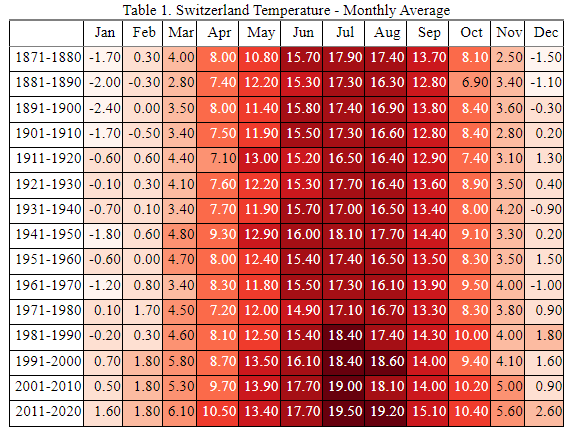
\includegraphics[scale=0.55]{heatmap.png}
    \end{minipage} 
\end{frame}


% ---------------------------------------------------------------------------
\begin{frame}{A Line Plot}
    \framesubtitle{Stock Performance}
    \begin{minipage}{\textwidth}
        \centering
        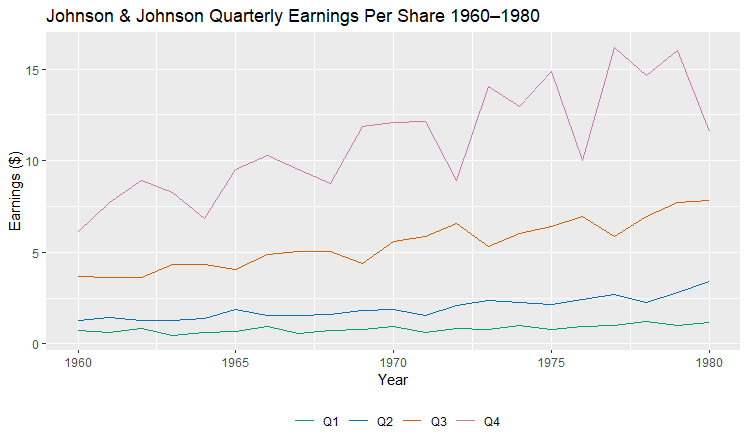
\includegraphics[scale=0.55]{lineplot.png}
    \end{minipage} 
\end{frame}

\end{document}

